\documentclass[12pt]{article}

% ---- Core packages ----
\usepackage[margin=1in]{geometry}
\usepackage{setspace}
\usepackage{xcolor}
\usepackage{graphicx}
\usepackage{titlesec}
\usepackage{fontspec}      % XeLaTeX/LuaLaTeX
\usepackage{fancyhdr}
\usepackage{enumitem}
\usepackage[strings]{underscore} % make _ safe in text and in arguments like \cite{...}
\usepackage{hyperref}             % load before biblatex
\usepackage{booktabs}

% ---- Bibliography: biblatex (modern, no natbib) ----
\usepackage[backend=biber,style=authoryear]{biblatex}
\addbibresource{references.bib}

% ---- Fonts (Overleaf has Roboto & Carlito) ----
\defaultfontfeatures{Ligatures=TeX}
\IfFontExistsTF{Roboto}{%
  \setmainfont{Roboto}%
}{%
  \setmainfont{Latin Modern Roman}%
}
\IfFontExistsTF{Roboto}{%
  \newfontfamily\robotosans{Roboto}[Scale=MatchLowercase]%
}{%
  \newfontfamily\robotosans{Latin Modern Sans}[Scale=MatchLowercase]%
}
\IfFontExistsTF{Carlito}{%
  \newfontfamily\carlito{Carlito}[Scale=MatchLowercase]%
}{%
  \newfontfamily\carlito{Latin Modern Sans}[Scale=MatchLowercase]%
}
% convenient alias
\newcommand{\roboto}{\robotosans}

% ---- Colors & section titles ----
\definecolor{projectblue}{HTML}{005F86}
\titleformat{\section}{\normalfont\color{projectblue}\bfseries\fontsize{22}{30}\selectfont}{\thesection.}{0.5em}{}
\titleformat{\subsection}{\normalfont\Large\bfseries}{\thesubsection}{0.5em}{}
\titleformat{\subsubsection}{\normalfont\large\bfseries}{\thesubsubsection}{0.5em}{}

% ---- Lists ----
\setlist[itemize]{leftmargin=1.2em}
\setlist[enumerate]{leftmargin=1.5em}

% ---- Inline code: safe for _, %, \, etc. ----
\newcommand{\inlinecode}[1]{\texttt{\detokenize{#1}}}

% ---- Header / footer ----
\setlength{\headheight}{32pt}
\pagestyle{fancy}
\fancyhf{}
\fancyhead[L]{%
    {\roboto\textbf{GROUP WORK PROJECT \# }1}\\
    {\roboto\textbf{Group Number: }11231}%
}
\fancyhead[R]{%
    {\carlito MScFE 600: FINANCIAL DATA}\\
}
\fancyfoot[C]{\thepage}

\begin{document}

\setcounter{section}{1}
\section{Yield Curve Modeling}

\bigskip

\subsection{Data Acquisition}
\begin{spacing}{1.15}
This section documents how the German government zero-coupon curve was sourced and validated as the foundation for the Nelson--Siegel and Cubic-Spline modeling tasks.

\subsubsection{Data Source and Coverage}
\begin{itemize}
    \item \textbf{Provider:} Deutsche Bundesbank SDMX REST API \parencite{bundesbank_rest_api}\\(dataset \inlinecode{D.I.ZST.ZI.EUR.S1311.B.A604}  \parencite{bundesbank_zero_coupon}.
    \item \textbf{Instrument set:} Zero-coupon yield curve for central government debt denominated in EUR.
    \item \textbf{Tenor breadth:} Residual maturities from 0.5 years (\inlinecode{R005X}) through 30 years (\inlinecode{R30XX}), covering each annual bucket in between. This satisfies the assignment requirement to span short- through long-term maturities (see the \emph{Description} section of \cite{bundesbank_zero_coupon}).
\end{itemize}

\subsubsection{Why the Bundesbank Term-Structure Series Dataset}
\begin{itemize}
  \item \textbf{Alignment with assignment scope:} The coursework requires a government-securities yield curve. Within the Bundesbank dataset catalog \parencite{bundesbank_data_yields}, the ``Term structure of interest rates in the debt securities market---estimated values'' \cite{bundesbank_zero_coupon} is the only branch that delivers a full maturity ladder for \emph{federal - government} securities.
  \item \textbf{Daily frequency and audit trail:} The ``Listed Federal securities'' subcategory exposes daily values for each maturity, letting us capture the most recent business day and preserve a reproducible cache.
  \item \textbf{Ready-to-use zero-coupon points:} The published Nelson--Siegel--Svensson estimates provide desmoothed spot rates at residual maturities from 0.5 to 30 years. Using these points avoids manual bond stripping while giving a clean target for the Nelson--Siegel and Cubic-Spline models that we must implement.
  \item \textbf{Alternative categories ruled out:} Money-market and deposit-rate tables do not cover government bonds; per-ISIN price tables require custom stripping; The Pfandbriefe pertain to covered bonds, not sovereign issuance. The \emph{Description} section in \cite{bundesbank_zero_coupon} confirms that the SDMX key \inlinecode{D.I.ZST.ZI.EUR.S1311.B.A604} targets the desired government curve.
\end{itemize}

\subsubsection{Retrieval Workflow}
\begin{enumerate}
    \item Determine the candidate business date in the \inlinecode{Europe/Berlin} timezone. If the current calendar day is a weekend or German public holiday, walk back to the previous business day using the official holiday calendar (\inlinecode{holidays.Germany}).
    \item For each maturity code in the published Bundesbank metadata, construct the full key of the SDMX series for each residual maturity and request the corresponding CSV slice for the target date, instead of fetching the whole dataset \parencite{bundesbank_zero_coupon_download}.
    \item Parse the returned CSV, drop metadata rows, and coerce the values to floats. If any tenor is missing or marked ``No value available'', record the gap and continue checking.
    \item Abort the fetch if any maturities are absent after iterating the full set. This guardrail prevents partially populated curves from contaminating downstream modelling.
\end{enumerate}

\subsubsection{Quality Controls and Audit Trail}
\begin{itemize}
    \item \textbf{Completeness checks:} The script raises an explicit error listing the missing maturities; the lookback window can be extended temporarily if necessary.
    \item \textbf{Caching:} Each successful run writes a timestamped snapshot to \inlinecode{data/raw/}, embedding both the curve date and the fetch timestamp to support reproduction and regulatory audit needs.
    \item \textbf{Reproducibility:} The notebook cell fetches data deterministically and without random sampling or manual intervention, ensuring that the fitted models can be regenerated on demand.
\end{itemize}

\end{spacing}

\subsection{Exploratory Analysis}
\begin{spacing}{1.15}
Figure~\ref{fig:raw-curve} shows the Bundesbank zero-coupon curve for 9 October 2025, exhibiting a gently upward-sloping structure that flattens beyond the 20-year point. Short-term yields remain below 2\%, while the long end stabilises around 3.3\%. Table~\ref{tab:summary-stats} summarises the cross-sectional statistics, confirming broad maturity coverage and moderate dispersion of yields. These diagnostics provide a clean baseline for parametric and non-parametric fits.
\end{spacing}

\begin{figure}[htbp]
  \centering
  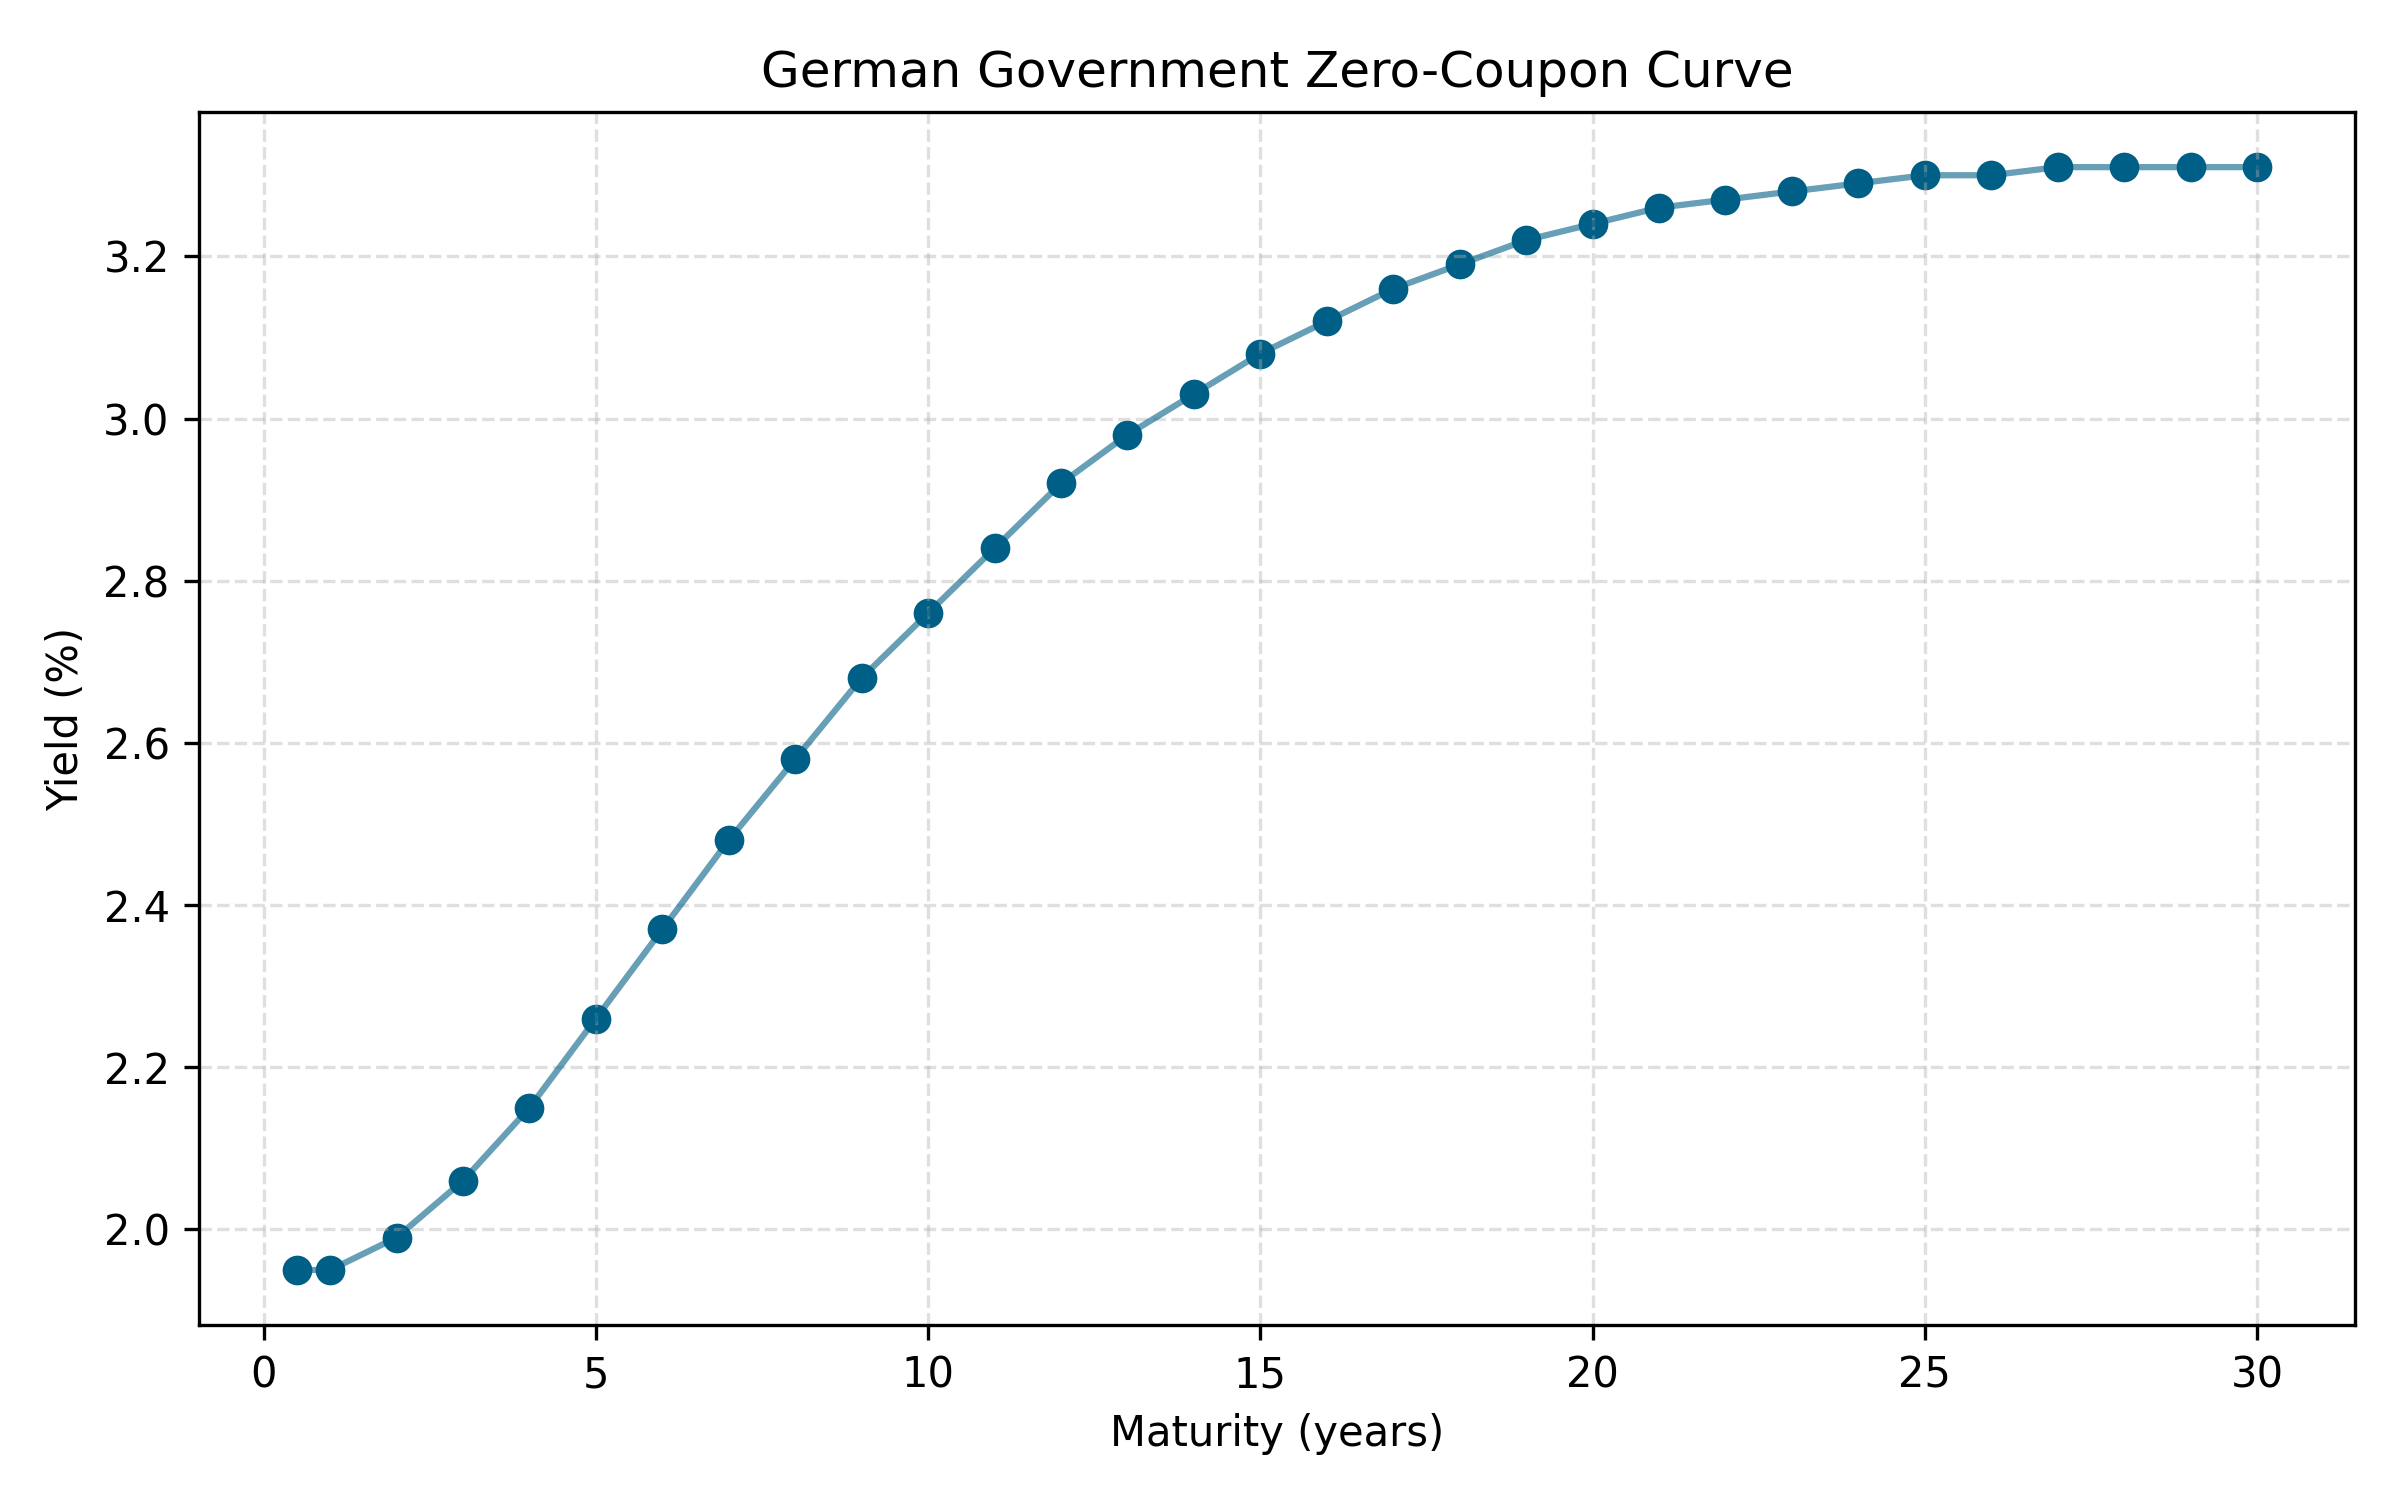
\includegraphics[width=0.8\textwidth]{../data/output/figure_raw_curve.png}
  \caption{Bundesbank zero-coupon yields by residual maturity on 9~October~2025. Source: \parencite{bundesbank_zero_coupon}.}
  \label{fig:raw-curve}
\end{figure}

\begin{table}[htbp]
  \centering
  \caption{Summary statistics for maturities and yields (9~October~2025).}
  \label{tab:summary-stats}
  \begin{tabular}{lrrrr}
\toprule
 & mean & std & min & max \\
\midrule
maturity_years & 15.0161 & 9.0650 & 0.5000 & 30.0000 \\
yield_pct & 2.8694 & 0.4811 & 1.9500 & 3.3100 \\
\bottomrule
\end{tabular}

\end{table}

\subsection{Nelson--Siegel Model}
\begin{spacing}{1.15}
We calibrate the four-parameter Nelson--Siegel (NS) specification \parencite{nelson_siegel_1987}, in which the spot rate at maturity $\tau$ is
\begin{equation}
  y_{\text{NS}}(\tau) = \beta_0 + \beta_1 \frac{1 - e^{-\tau/\tau_1}}{\tau/\tau_1} + \beta_2 \left( \frac{1 - e^{-\tau/\tau_1}}{\tau/\tau_1} - e^{-\tau/\tau_1} \right).
\end{equation}
The factors $(\beta_0, \beta_1, \beta_2)$ capture the level, slope, and medium-term curvature respectively, while $\tau_1$ controls the decay of the exponential loading. Parameters are estimated with non-linear least squares against the 0.5--30 year cross-section. The fitted curve (Figure~\ref{fig:ns-fit}) follows the broad shape of the data but leaves residual structure at both extremes, signalling the need for additional flexibility.

Table~\ref{tab:param-summary} reports the calibrated coefficients. The level factor $\beta_0$ settles near 3.68\%, consistent with long-dated yields, whereas the negative slope factor reflects the downward tilt between the short and long ends observed in the data.
\end{spacing}

\begin{figure}[htbp]
  \centering
  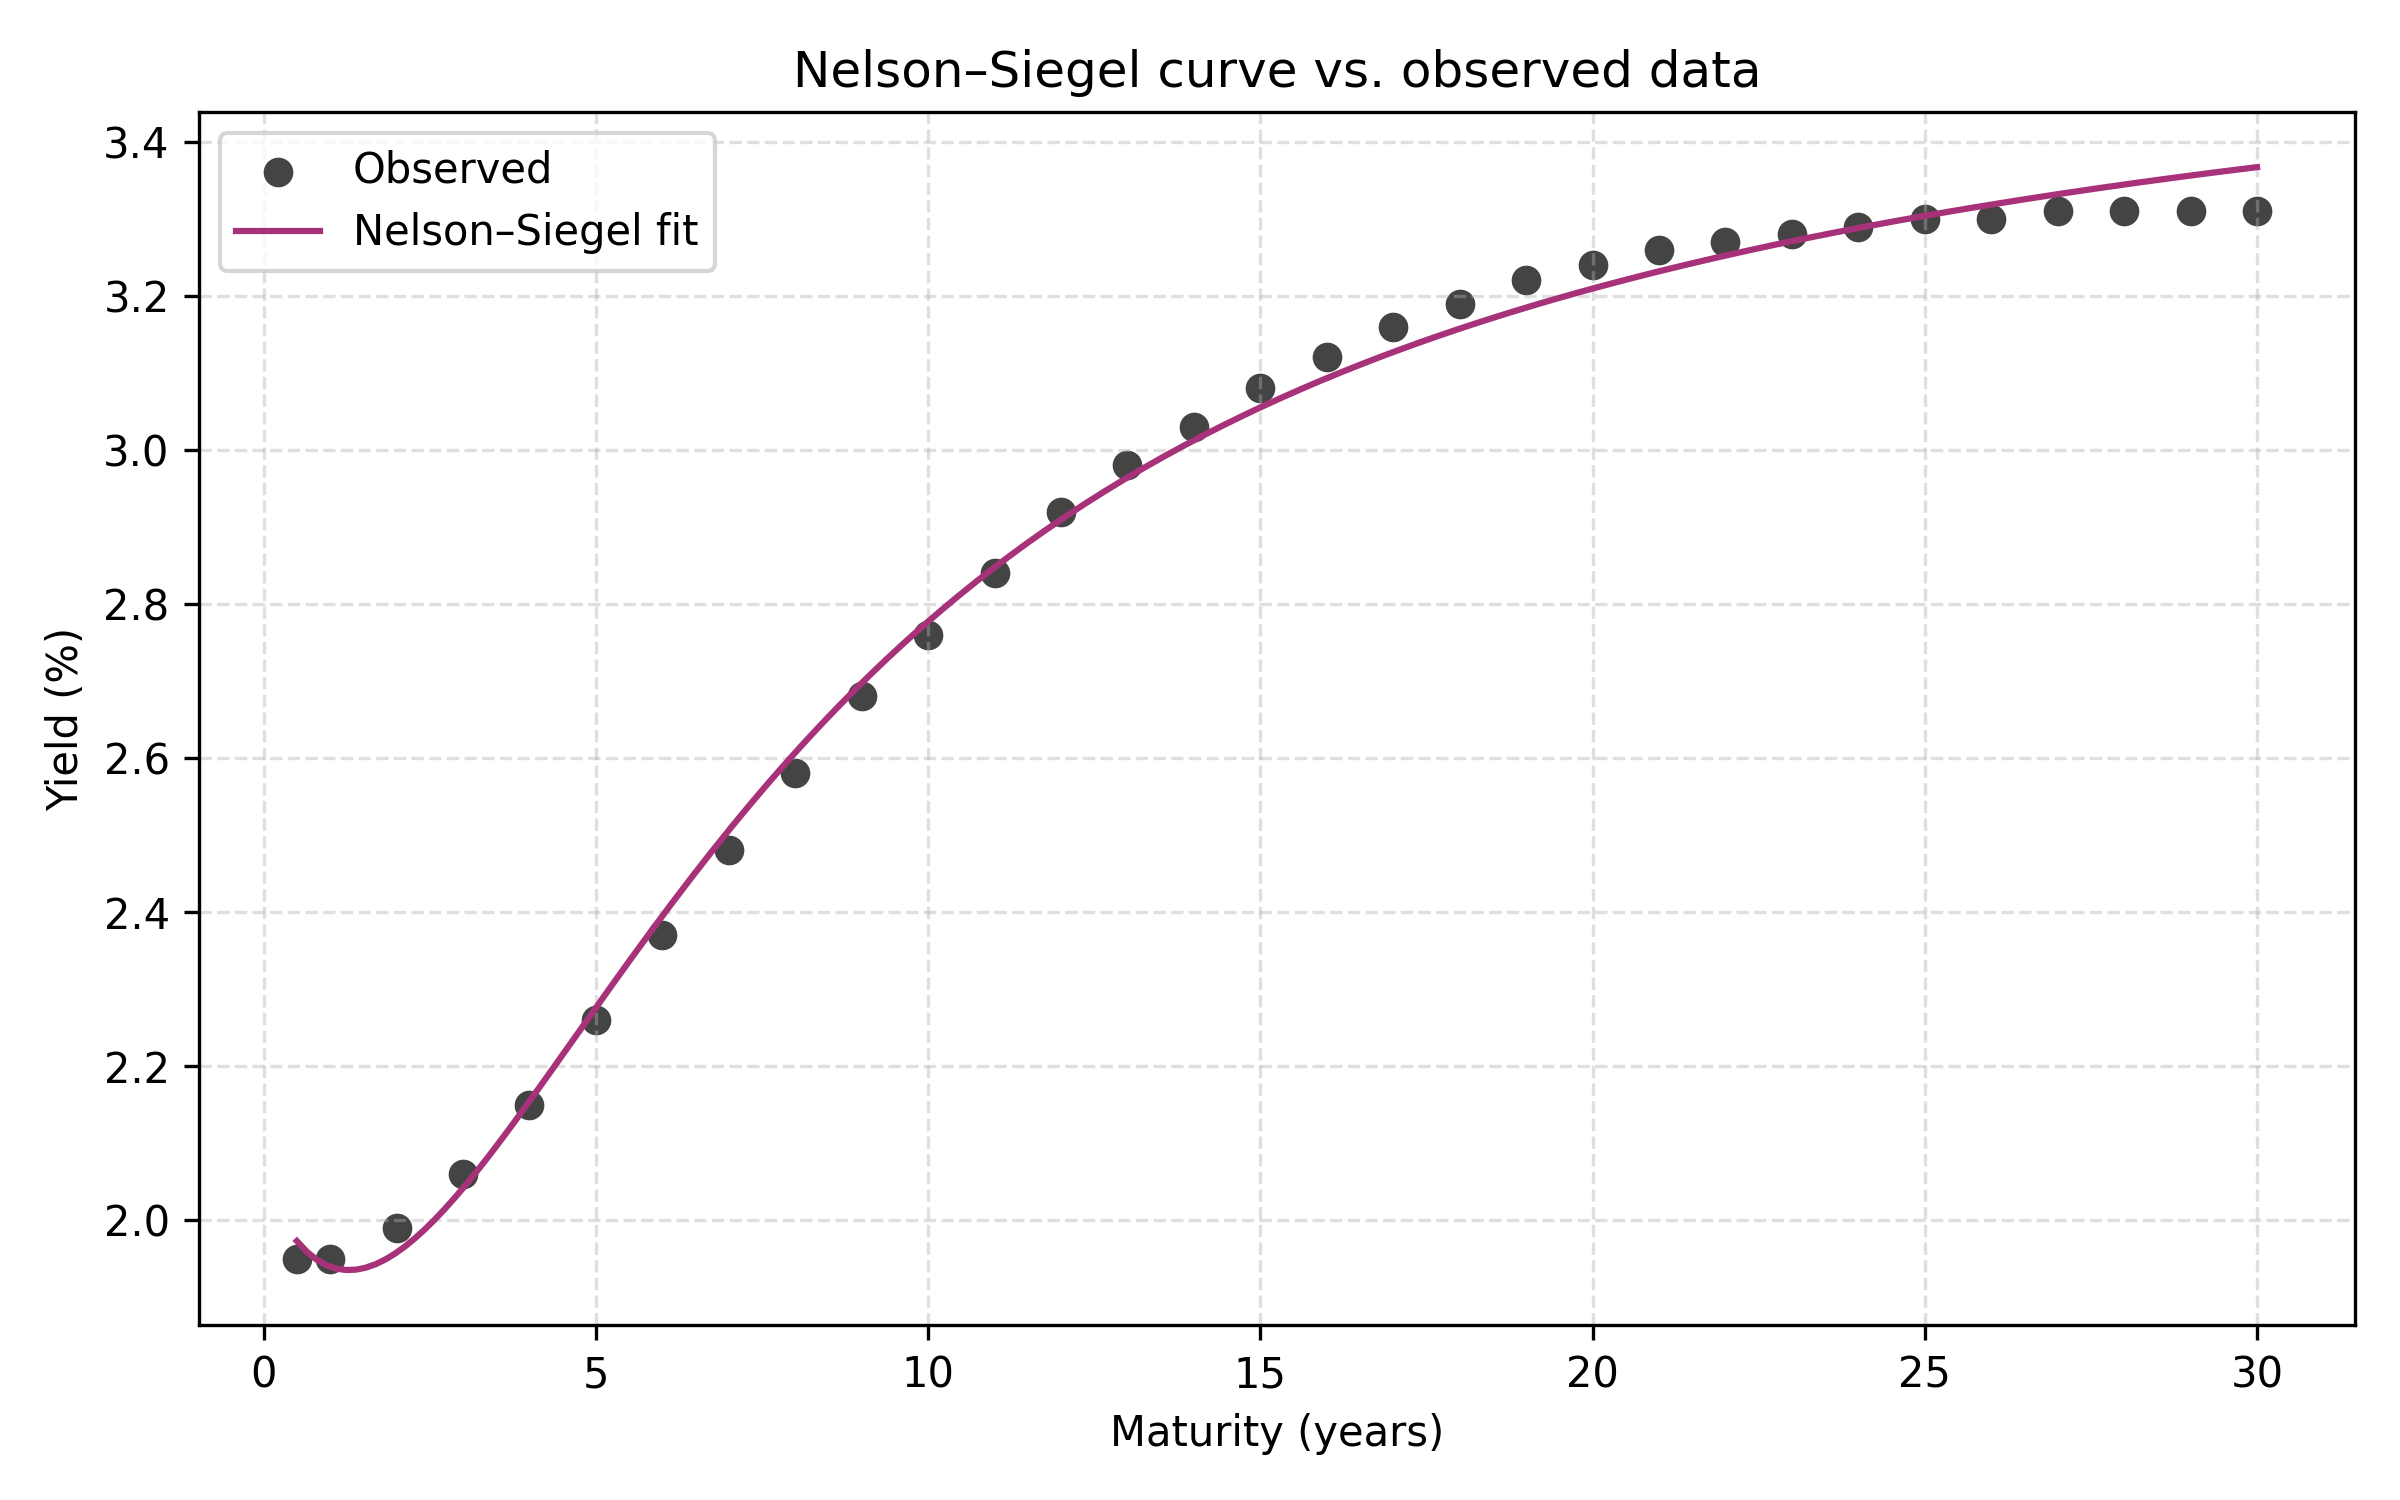
\includegraphics[width=0.8\textwidth]{../data/output/figure_ns_fit.png}
  \caption{Nelson--Siegel fit versus observed yields.}
  \label{fig:ns-fit}
\end{figure}

\subsection{Nelson--Siegel--Svensson Extension}
\begin{spacing}{1.15}
To capture long-end curvature we extend the model with the Nelson--Siegel--Svensson (NSS) term \parencite{diebold_li_2006, ecb_yield_curve_2018}. The NSS curve augments the NS structure with an additional exponential hump:
\begin{equation}
  y_{\text{NSS}}(\tau) = y_{\text{NS}}(\tau) + \beta_3 \left( \frac{1 - e^{-\tau/\tau_2}}{\tau/\tau_2} - e^{-\tau/\tau_2} \right),
\end{equation}
introducing parameters $(\beta_3, \tau_2)$ that target long-term dynamics. Figure~\ref{fig:nss-fit} illustrates the near-perfect alignment between NSS estimates and observed yields; the additional curvature term corrects the slight under- and over-shoots left by the NS curve. Parameter values in Table~\ref{tab:param-summary} show how $\beta_3$ adds a second hump around eight years, while $\tau_1$ shifts upward to focus the original curvature on the mid-belly.
\end{spacing}

\begin{figure}[htbp]
  \centering
  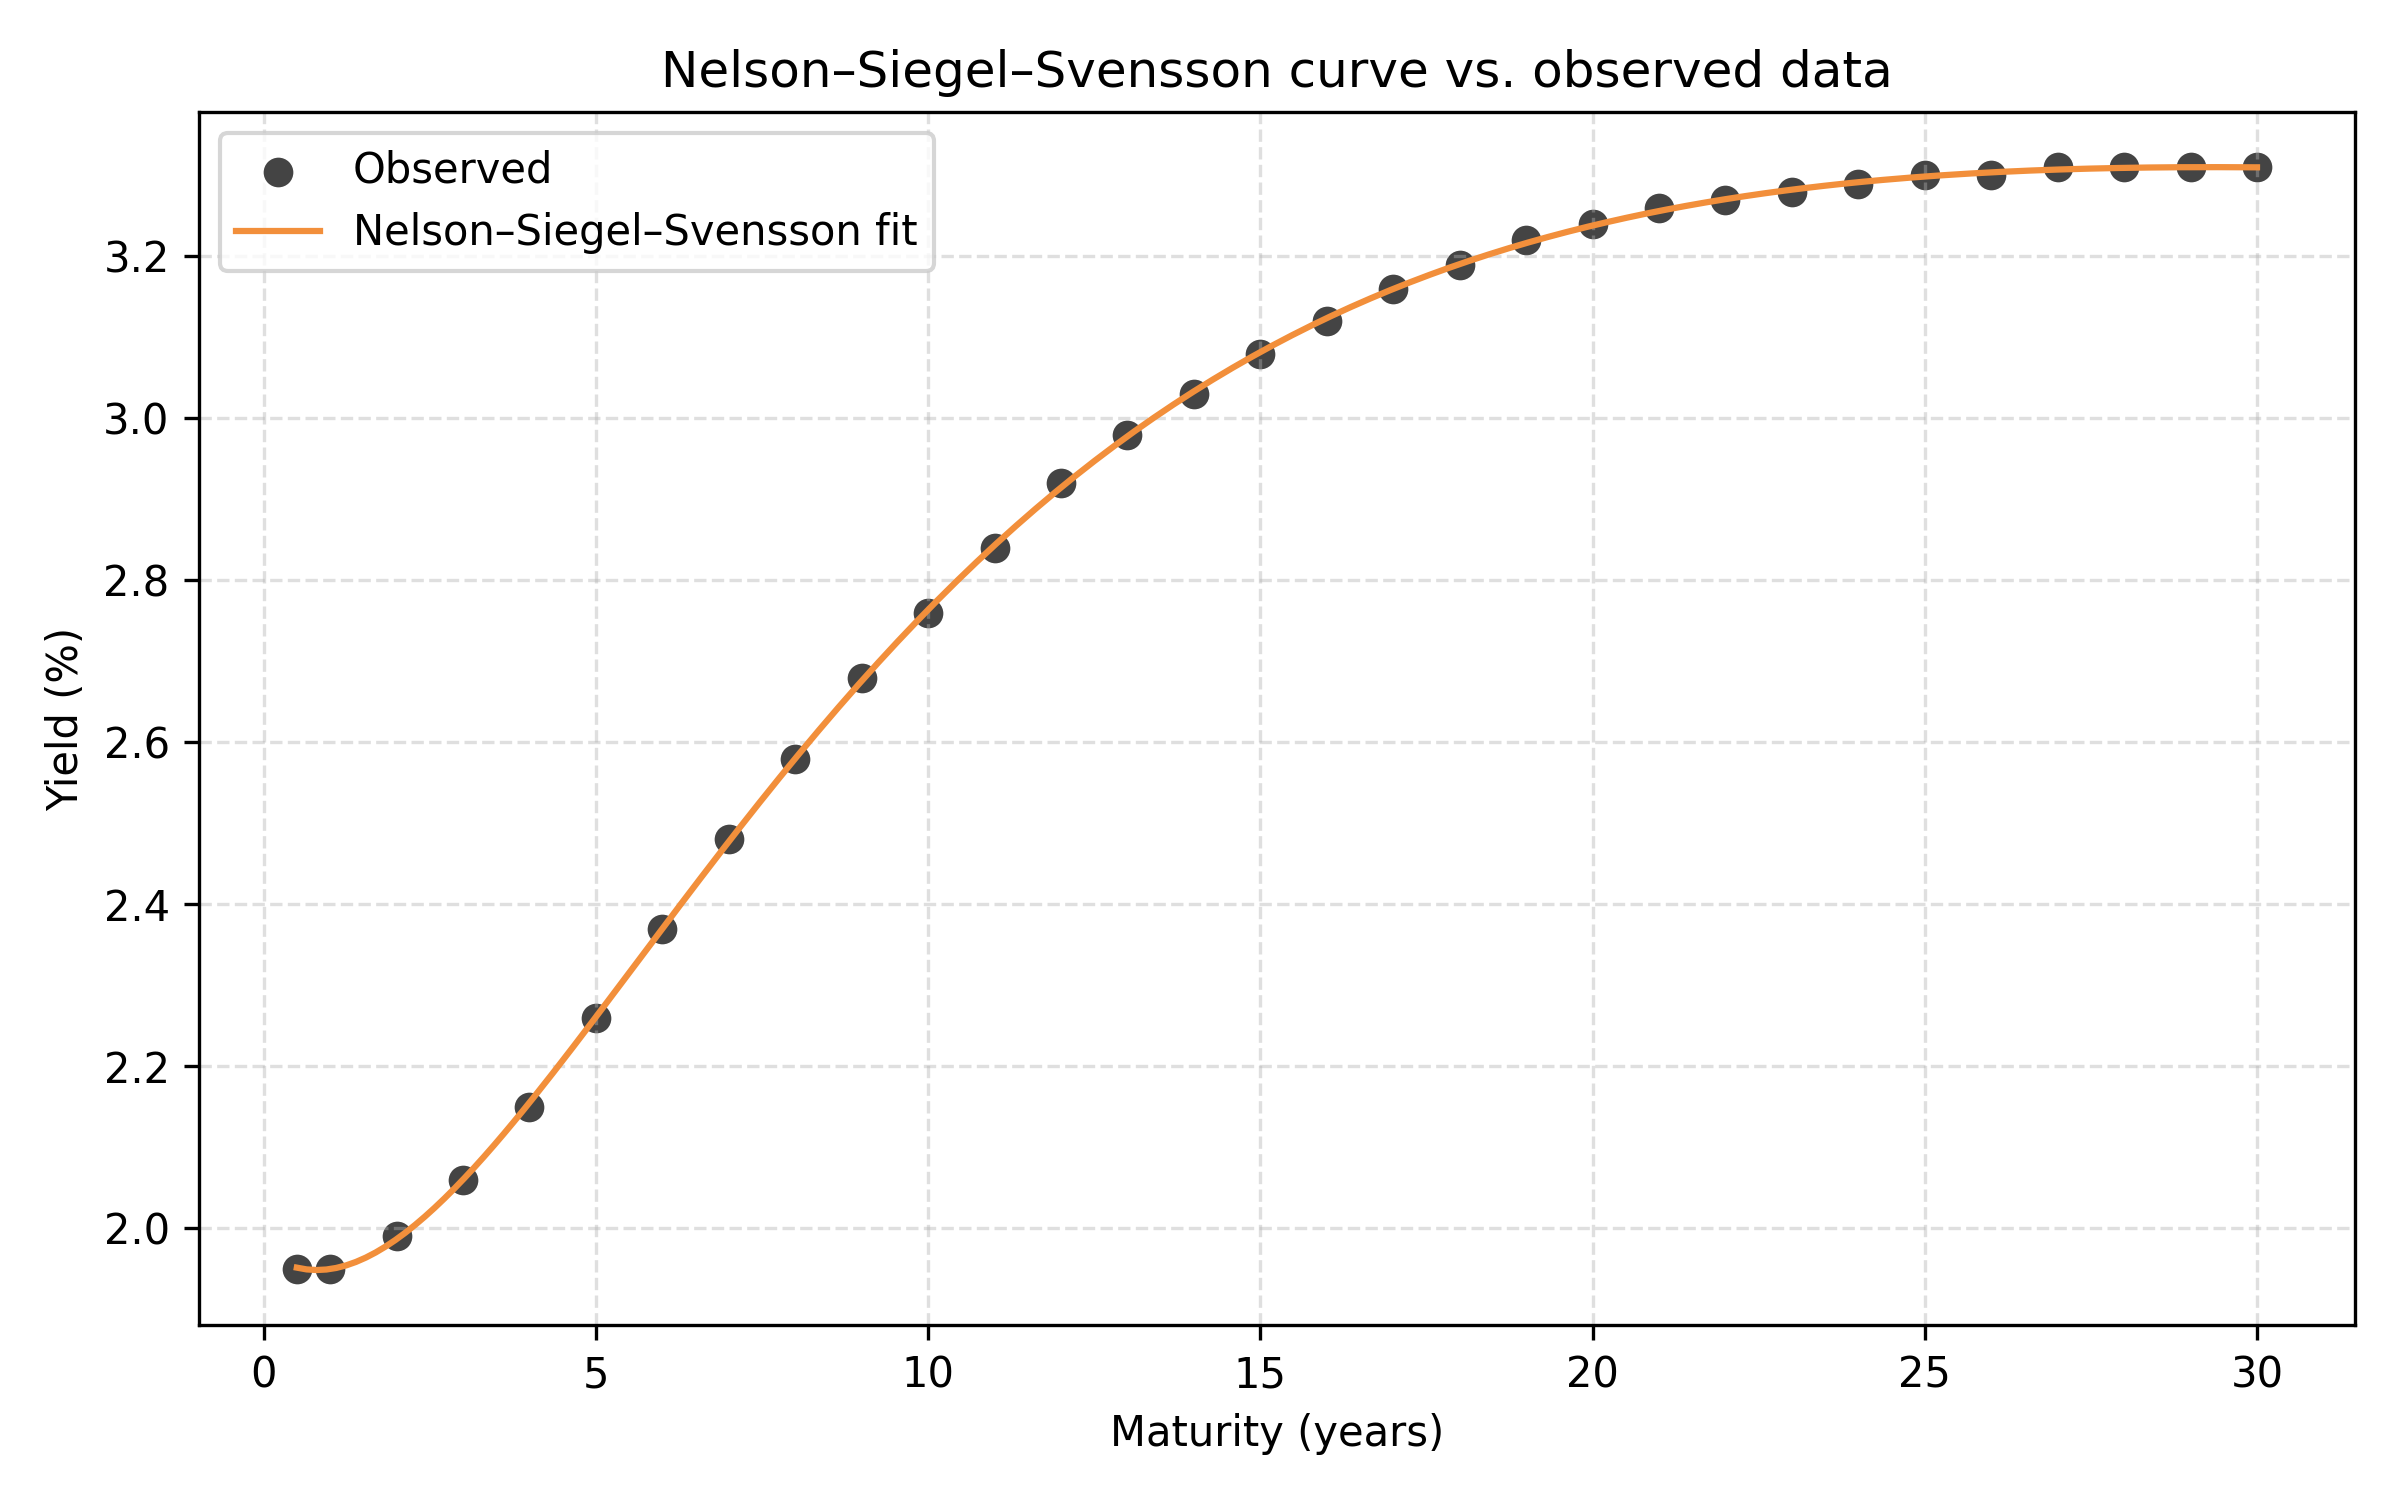
\includegraphics[width=0.8\textwidth]{../data/output/figure_nss_fit.png}
  \caption{Nelson--Siegel--Svensson fit versus observed yields.}
  \label{fig:nss-fit}
\end{figure}

\subsection{Cubic Spline Model}
\begin{spacing}{1.15}
As a flexible benchmark we fit a smoothing spline through the same maturity-yield pairs. The spline captures local curvature without imposing an explicit factor structure, making it suitable for interpolation when parametric assumptions are suspect. Figure~\ref{fig:spline-fit} demonstrates the excellent in-sample alignment, although the method lacks interpretable parameters.
\end{spacing}

\begin{figure}[htbp]
  \centering
  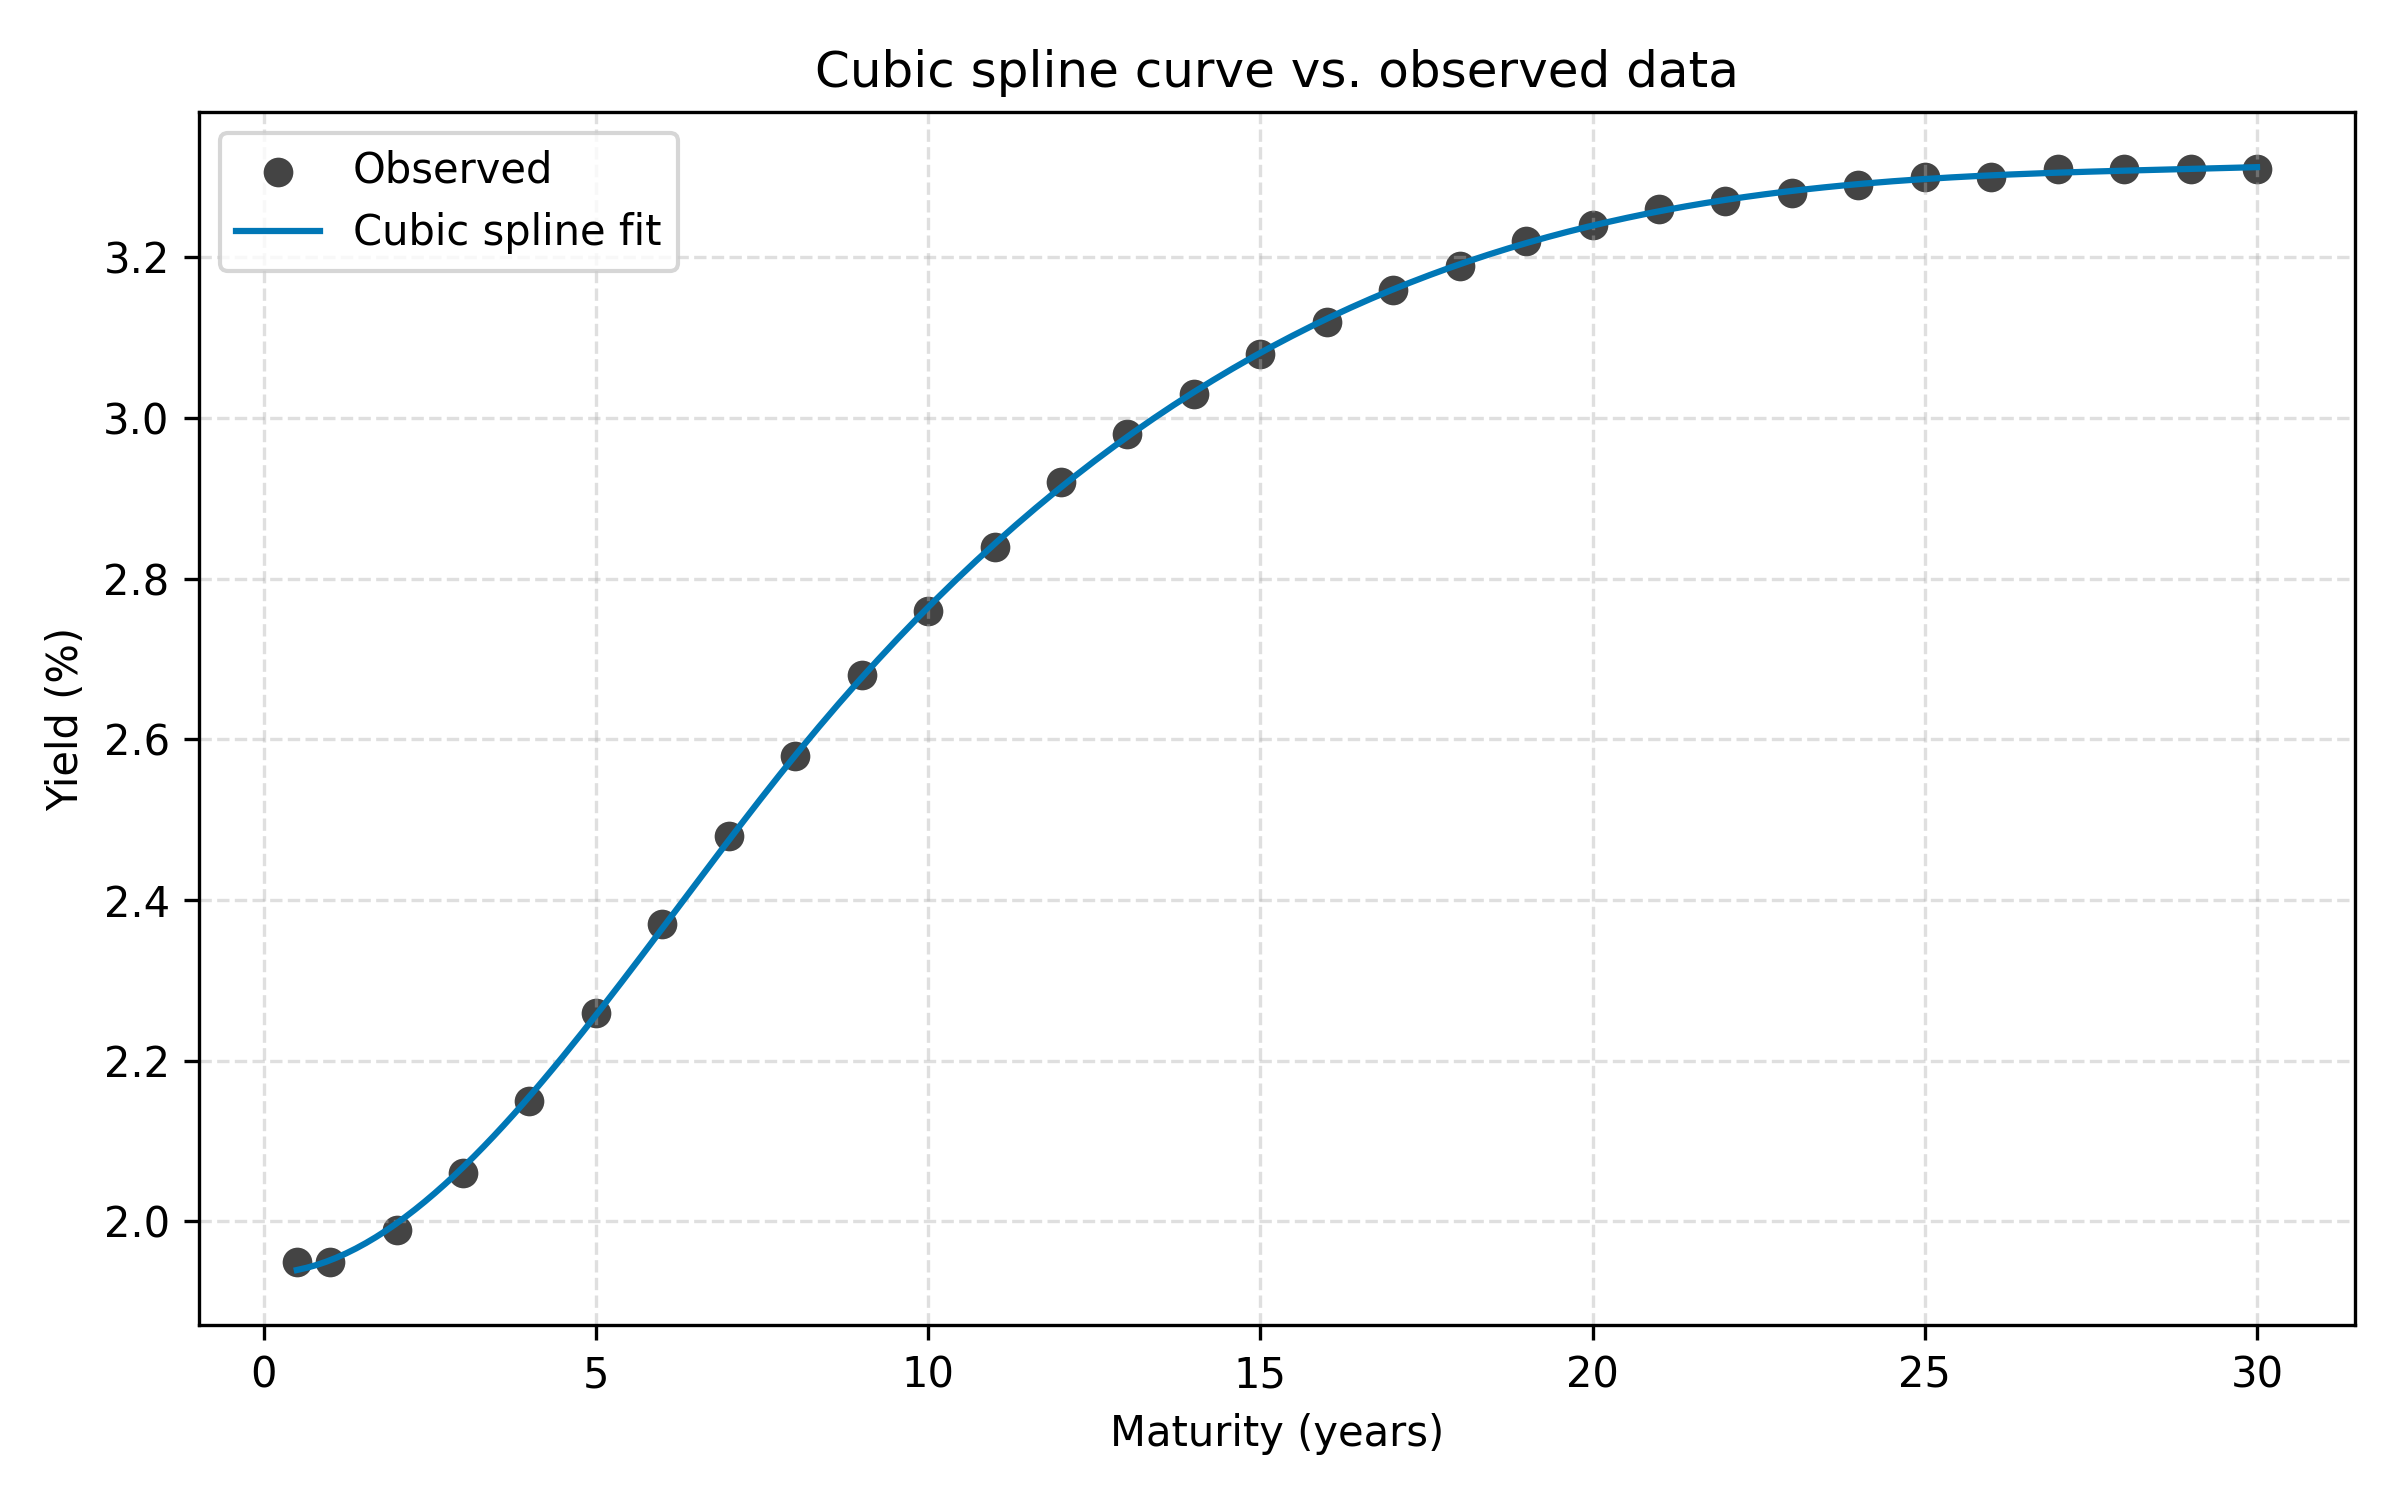
\includegraphics[width=0.8\textwidth]{../data/output/figure_spline_fit.png}
  \caption{Cubic spline fit versus observed yields.}
  \label{fig:spline-fit}
\end{figure}

\subsection{Model Comparison and Ethics}
\begin{spacing}{1.15}
Table~\ref{tab:model-metrics} contrasts root-mean-square and mean-absolute residuals across all maturities. The NSS specification delivers the lowest errors, followed closely by the spline, while the base NS model under-fits the curve. Residual diagnostics in Figure~\ref{fig:residuals} confirm that NSS and the spline leave only basis-point level noise, whereas NS exhibits systematic deviations at both the short and long ends.

Crucially, NSS retains the interpretability of factor loadings. Table~\ref{tab:param-summary} shows that adding $(\beta_3, \tau_2)$ reallocates curvature to the long end without abandoning the economic meaning of level, slope, and medium-term hump factors. The spline, by contrast, offers no parameter-level narrative despite its competitive fit.

In light of Module~2 Lesson~4 discussions, smoothing via Nelson--Siegel-type models is not inherently unethical provided the methodology and residual diagnostics are disclosed. Our workflow publishes parameter estimates, error metrics, and residual plots alongside the raw Bundesbank points, ensuring stakeholders can gauge any discrepancies rather than relying on a black-box smoother.
\end{spacing}

\begin{table}[htbp]
  \centering
  \caption{Parameter estimates for the fitted term-structure models.}
  \label{tab:param-summary}
  \begin{tabular}{lrrrrrr}
\toprule
 & β₀ (level) & β₁ (slope) & β₂ (curvature) & β₃ (long curvature) & τ₁ (decay) & τ₂ (long decay) \\
\midrule
Nelson–Siegel & 3.6833 & -1.6349 & -2.5519 &  & 2.2657 &  \\
Nelson–Siegel–Svensson & 2.9598 & -0.9889 & -2.9529 & 3.4375 & 3.6973 & 8.3372 \\
Cubic spline &  &  &  &  &  &  \\
\bottomrule
\end{tabular}

\end{table}

\begin{table}[htbp]
  \centering
  \caption{Fit diagnostics (percentage-point units).}
  \label{tab:model-metrics}
  \begin{tabular}{lrr}
\toprule
 & RMSE & MAE \\
\midrule
Nelson–Siegel & 0.0253 & 0.0222 \\
Nelson–Siegel–Svensson & 0.0027 & 0.0021 \\
Cubic spline & 0.0040 & 0.0033 \\
\bottomrule
\end{tabular}

\end{table}

\begin{figure}[htbp]
  \centering
  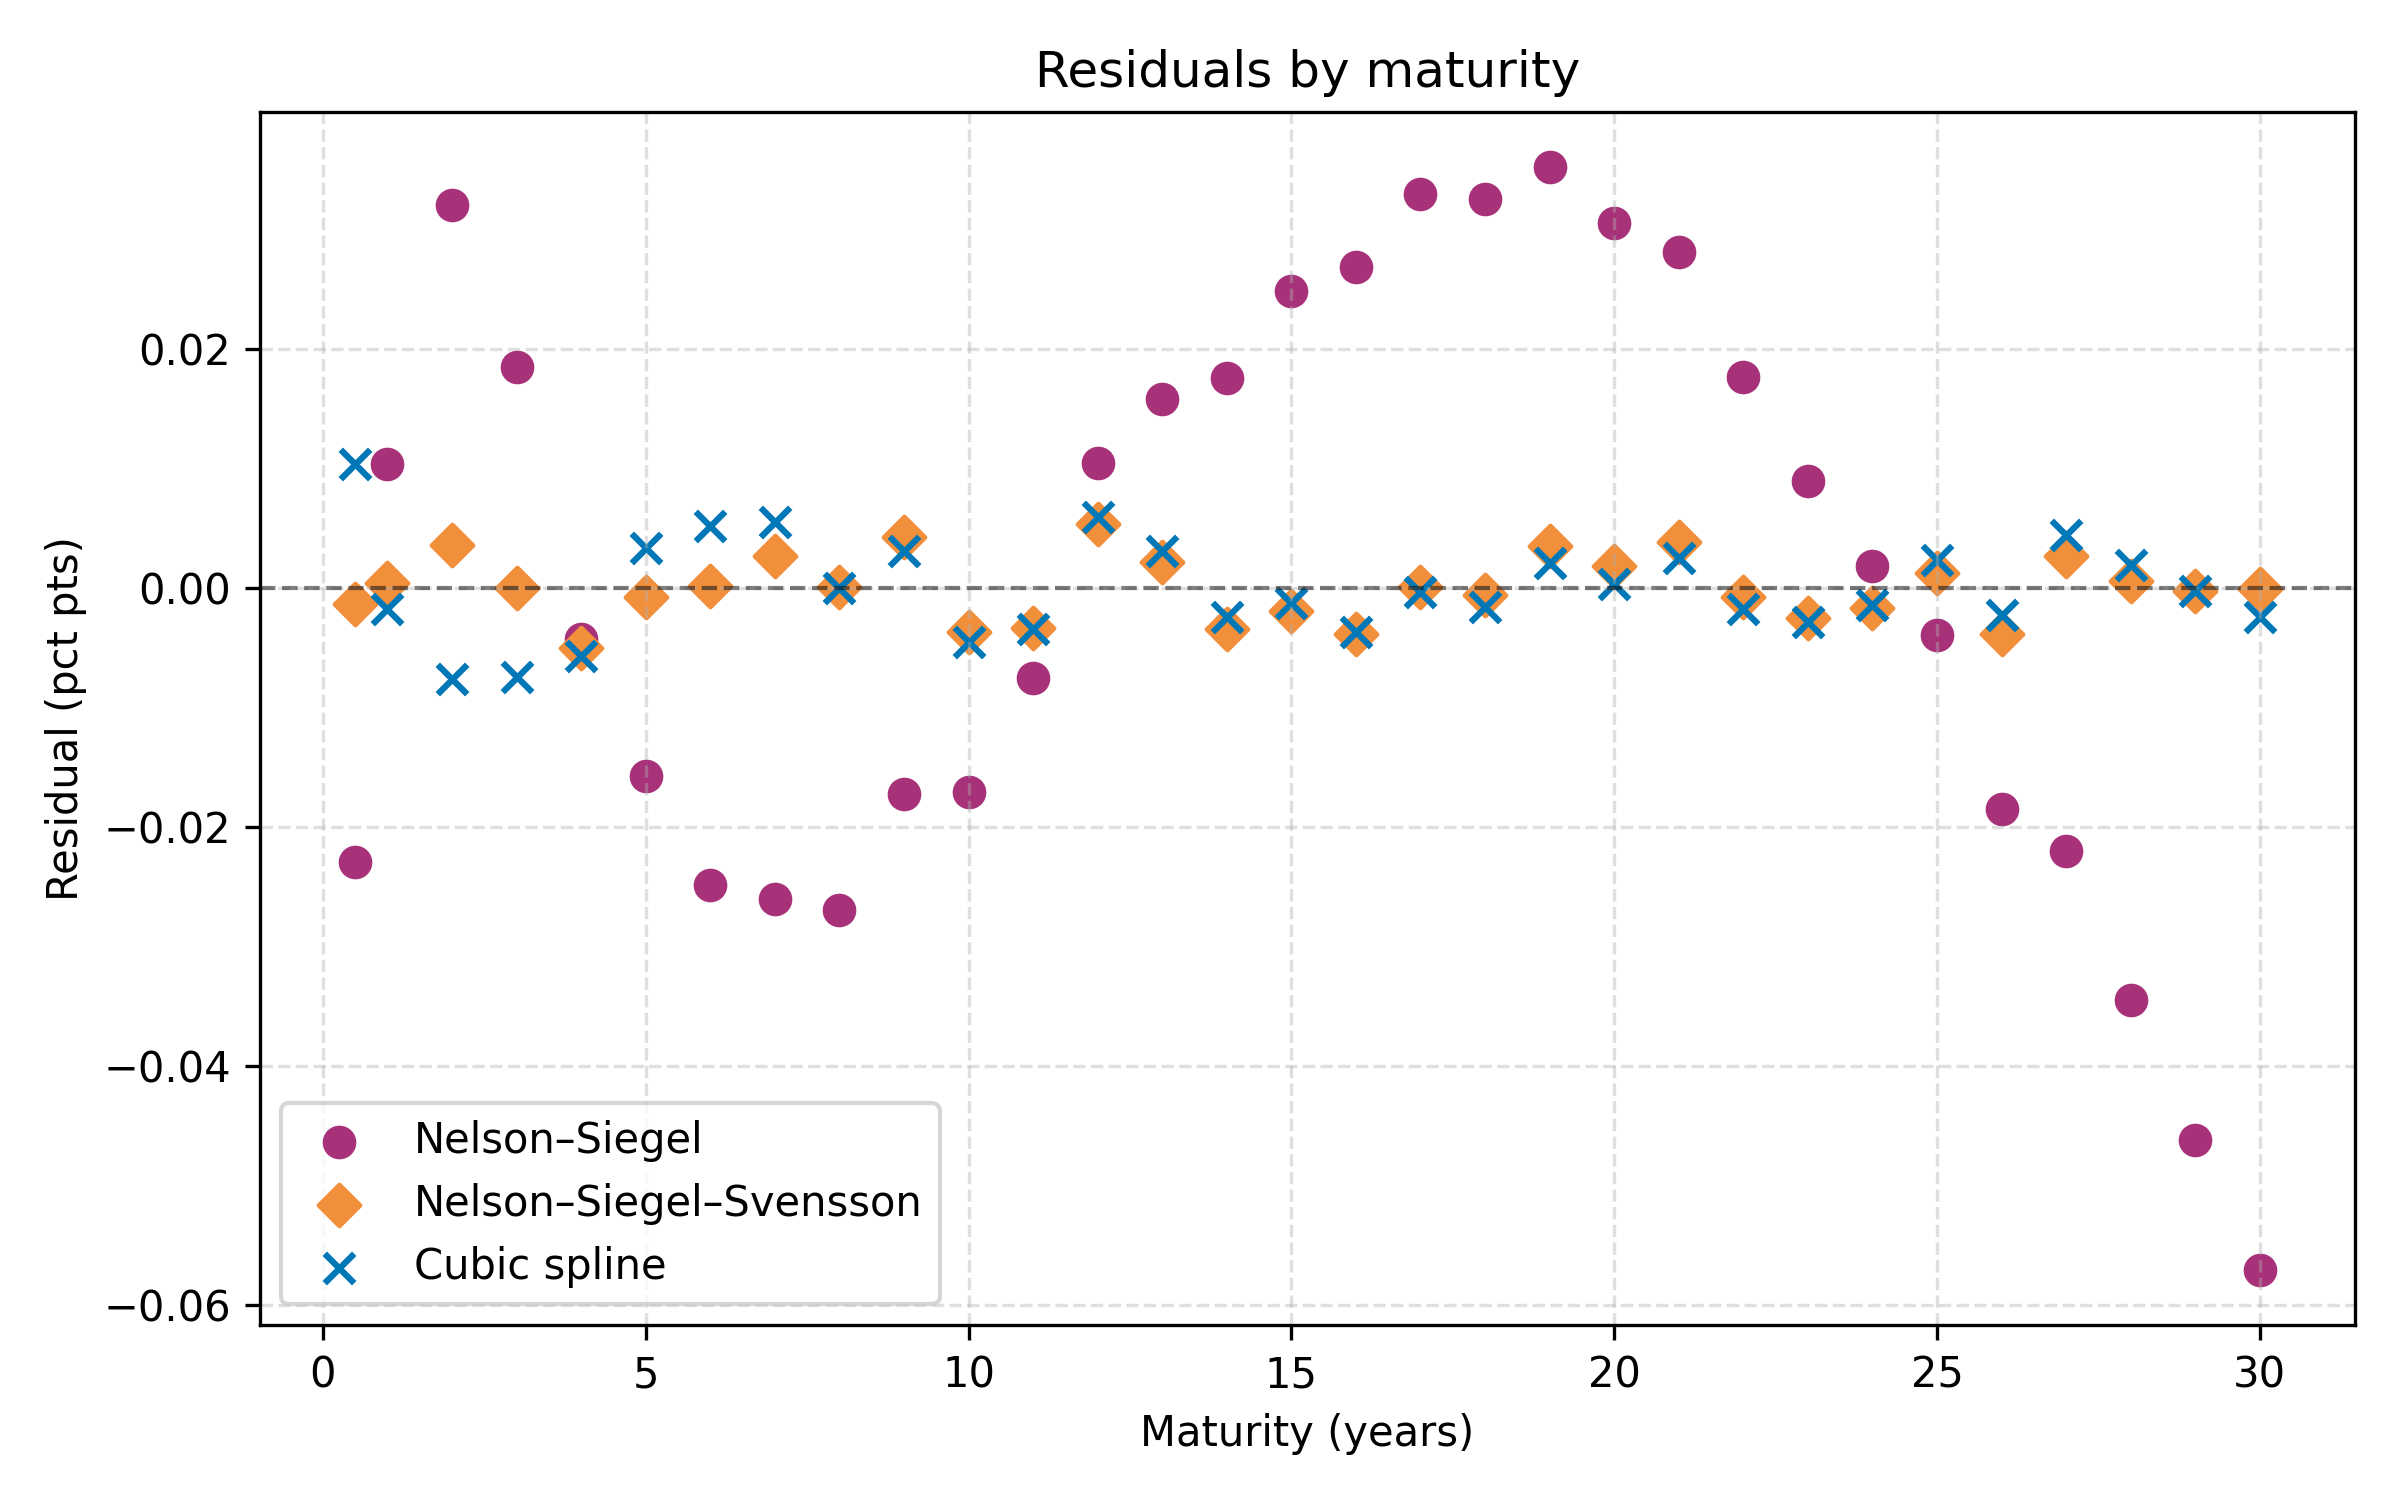
\includegraphics[width=0.8\textwidth]{../data/output/figure_model_residuals.png}
  \caption{Residuals by maturity for NS, NSS, and spline fits.}
  \label{fig:residuals}
\end{figure}

\printbibliography

\end{document}
